\label{sec:confounder-audits}

\subsection{PTEN and AR: does grade explain everything?}

For markers 4 and 6, a fully nested clinical-only / image-only / combined comparison tests
held-out incremental value beyond Gleason grade (Table~\ref{tab:confounder-4-6},
Figure~\ref{fig:confounder-audit}a; the same design applied to marker 7 is deferred to
Section~\ref{sec:recurrence-transfer}, since that marker's story is inseparable from the
downstream-transfer question). The results are materially weaker than the auxiliary in-sample
analyses described in Section~\ref{sec:gate4-methods}. PTEN's patient-level $\Delta$AUROC is
$+0.019$ (bootstrap 95\% CI $[-0.025,+0.068]$; fully refit permutation $p=0.203$), and AR's
$\Delta R^2$ is $+0.004$ ($[-0.036,+0.042]$; $p=0.176$). Neither supports a confident
grade-adjusted held-out increment. The earlier full-cohort LRT/fixed-score permutation results
remain positive (PTEN $p=0.010/0.014$; AR $p=0.003/0.0025$), but are retained only as
explicitly in-sample/fixed-score auxiliary analyses; their disagreement with nested refitting
is itself the reason to prefer the latter.

Because this project has repeatedly found CONCH and Virchow disagree on individual results
(most sharply for marker 7's zero-shot transfer, Section~\ref{sec:recurrence-transfer}), a
single-encoder nested result is not yet the strongest available evidence, so we re-ran the same
nested bootstrap pipeline on Virchow embeddings for PTEN and AR (marker 7 was not re-audited
in this analysis; its endpoint/encoder/scale-limited transfer interpretation is instead bounded
by the completed common-498 R2, official-PFI R3, and paired R4 analyses). Virchow
\emph{converges} with CONCH rather than diverging: PTEN's held-out $\Delta$AUROC is $+0.035$
(95\% CI $[-0.013,+0.087]$) and AR's $\Delta R^2$ is $+0.019$ ($[-0.015,+0.051]$) -- both
small, both positive in direction, and both intervals crossing zero, the same qualitative
pattern as CONCH. Agreement between two independently trained encoders on a \emph{weak,
uncertain} result is itself informative: it argues the small nested increment is a property of
the underlying grade--PTEN/AR relationship rather than an artifact specific to CONCH's
embedding space.

Figure~\ref{fig:confounder-audit}b shows AR's unresolved site transportability as a forest plot.
The six eligible sites contain 224 slides and 209 patients; patient-level site median AR
activity ranges from $-3.46$ (YL) to $+1.71$ (EJ). The displayed leave-one-site-out effect is,
however, a \emph{slide-level} Spearman correlation with a patient-cluster bootstrap 95\% CI,
whereas the pooled $\rho=+0.195$ [0.07, 0.31] is patient-level internal-CV performance. The six
leave-one-site-out point estimates range from $\rho=-0.13$ (CH) to $+0.27$ (KK), and every
interval includes zero. Thus neither the differing site descriptors nor the sign pattern
supports or refutes site heterogeneity or transportability. Separately, all 60 Gate A
seed-level cells are positive ($\rho=0.136$--$0.297$), so AR's positive pooled direction is
consistent across the correlated Gate A settings; the nested results still leave the
grade-independent increment unresolved.

The R5 page-0 header inventory completed all 300 slides. It records a raw ScanScope ID for
280/300 slides and an explicit stain field for 0/300. A raw ScanScope identifier is not a
scanner-model annotation, and its distribution remains entangled with tissue-source site;
stain metadata are unavailable rather than inferred. Consequently these metadata cannot
separate scanner or stain from site. No scanner, stain, or site causality is inferred. C05
evidence closure is complete, while the scientific question remains unresolved.

\begin{figure}[htbp]
\centering
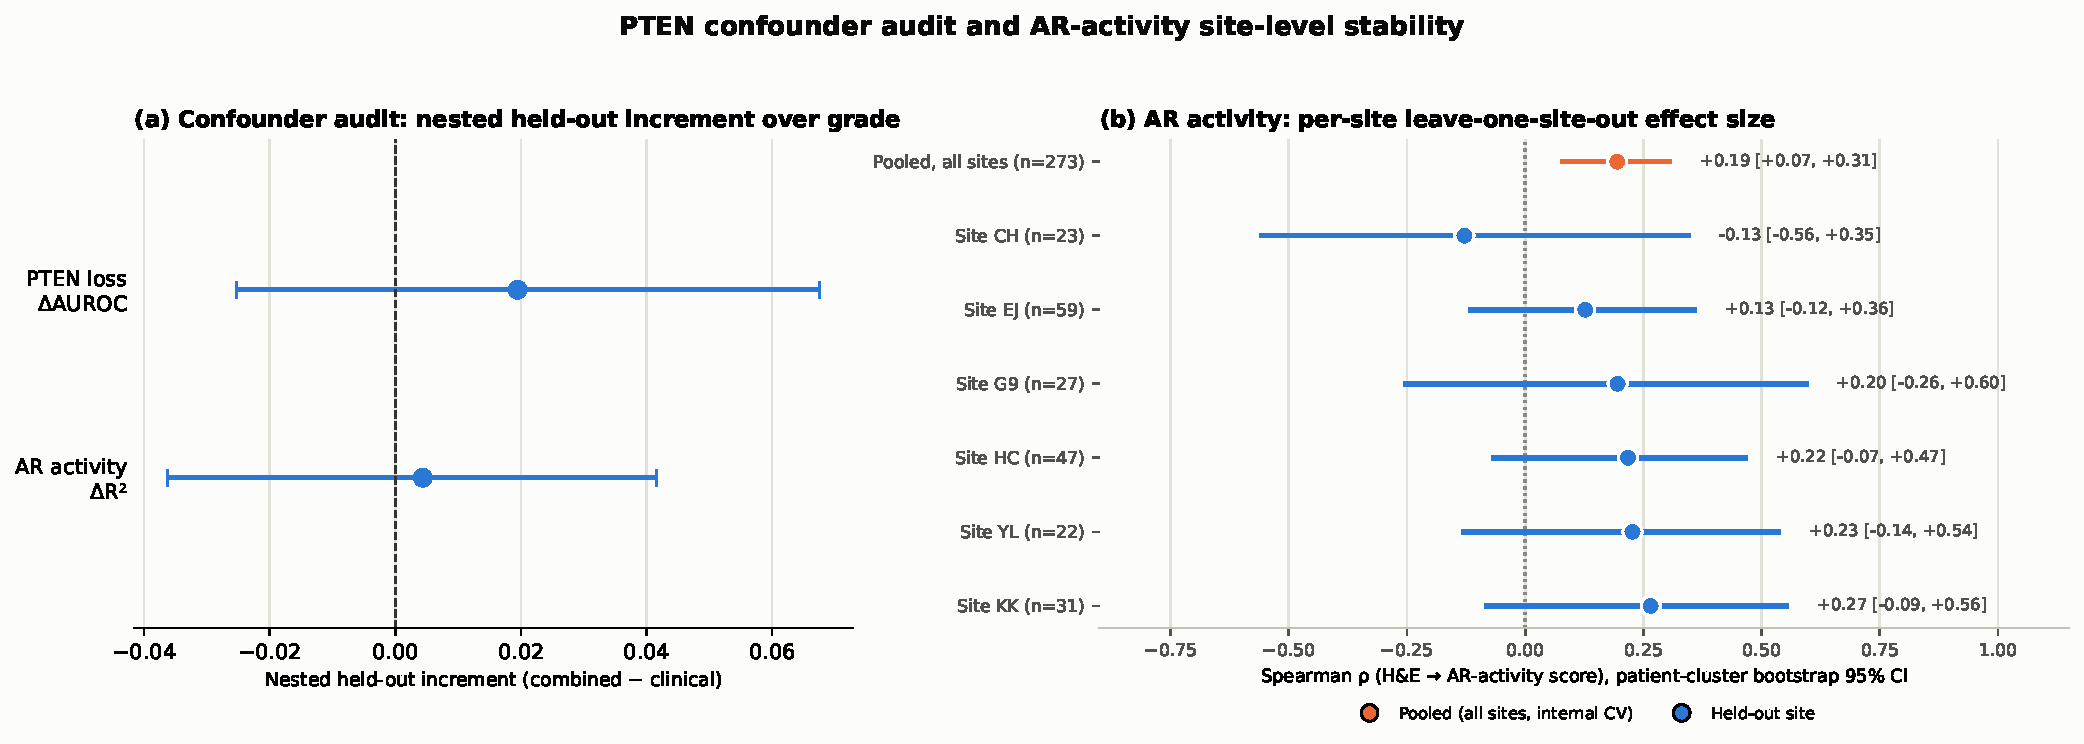
\includegraphics[width=0.95\textwidth]{figures/fig6_pten_ar_confounder.pdf}
\caption{(a) Nested held-out confounder-audit increment for PTEN and AR (combined $-$ clinical),
patient-bootstrap 95\% CI. (b) AR-activity per-site leave-one-site-out effect size vs.\ the
pooled all-sites internal-CV estimate.}
\label{fig:confounder-audit}
\end{figure}

TCGA multi-assay concordance (PTEN copy-number loss vs.\ mRNA expression vs.\ RPPA protein
level, all measured independently) further supports PTEN as the strongest-triangulated marker
in the pool ($p=7.8\times10^{-30}$ CNA-loss vs.\ mRNA, $p=0.001$ CNA-loss vs.\ RPPA), while
confirming AR's three assay layers are correlated but, as previously characterized, not fully
independent (all three are partly RNA-derived).

\begin{table}[htbp]
\centering
\small
\begin{tabular}{lcccccc}
\toprule
Marker & Clinical & Image & Combined & $\Delta$ & 95\% CI & Refit $p$ \\
\midrule
PTEN loss (AUROC) & 0.596 & 0.632 & 0.615 & $+0.019$ & [$-0.025$, 0.068] & 0.203 \\
AR activity ($R^2$) & $-0.003$ & $+0.024$ & $+0.001$ & $+0.004$ & [$-0.036$, 0.042] & 0.176 \\
\bottomrule
\end{tabular}
\caption{Nested held-out confounder audit for PTEN and AR. Metrics are patient-level outer-OOF
values; $\Delta$ is combined minus clinical, with paired patient-bootstrap intervals (2{,}000
resamples). Refit $p$ uses label permutation within rounded grade strata and repeats the
complete nested pipeline (2{,}000 requested repetitions). Marker 7's analogous table is
Table~\ref{tab:confounder-7}.}
\label{tab:confounder-4-6}
\end{table}

\subsection{SPOP: frozen-primary and configuration-sensitivity interpretation}

R5 retains all 22 tissue-source sites and distinguishes a historical slide-reportability rule
from whether patient AUROC is mathematically defined. Among the six sites with at least 20
slides, CH is undefined because all 23 patients are SPOP-negative. Patient AUROC is defined at
the other five sites: EJ 0.613, G9 0.700, HC 0.758, KK 0.573, and YL 0.625. G9, HC, and YL
have only 2, 3, and 4 positive patients, respectively, so their uncertainty is correspondingly
large; only EJ, KK, and YL satisfy the historical rule of at least five positive and five
negative \emph{slides}. Across CH/EJ/G9/HC/KK/YL, the 2,000-draw patient bootstrap preserves
2,000, 0, 234, 92, 2, and 31 undefined draws, respectively. Every defined interval includes
or touches 0.5.

We also checked whether the project's standard \texttt{class\_weight="balanced"} choice was itself
responsible for the primary near-chance estimate, since SPOP mutation prevalence is low (12\%, 36/300 slides).
Re-fitting with no class reweighting gives a nearly identical result (slide AUROC $0.506$ vs.\
$0.508$, patient AUROC $0.516$ vs.\ $0.519$, both non-significant either way) -- that primary
estimate is not an artifact of the class-imbalance handling choice. The balanced patient-level bootstrap
interval is $[0.408,0.627]$. A Hanley--McNeil fixed-score normal approximation places the
minimum detectable AUROC at 0.661 for 80\% power and 0.685 for 90\% power (two-sided
$\alpha=0.05$). These are planning approximations that omit probe-training uncertainty,
out-of-fold dependence, site heterogeneity, configuration selection, and multiplicity; they
are not an effect-exclusion bound. The completed Gate A grid broadens this caution: SPOP AUROC spans
0.348--0.679, with 25/60 chance-or-worse seed-level cells, 8/12 five-seed configurations whose
seed range straddles chance, 19/30 native-scale null crossings, and 4/15 shared-scale encoder
null crossings. SPOP is therefore unsupported in the frozen primary configuration and
configuration-sensitive in Gate A; neither a robust positive nor a robust null is established.
A modest effect and tumor dilution remain unresolved. C04 evidence closure is complete, but
the scientific interpretation remains unresolved; the source-driven details are shown in
Figure~\ref{fig:scale-heatmap} and Supplementary
Table~\ref{tab:supp-stability-grid}.
